\section{Task 2: Exploiting a Simple Buffer Overflow on the Stack}

\begin{figure}[H]
	\centering
	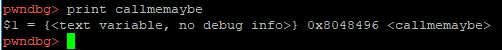
\includegraphics[width=0.8\textwidth]{Assignment0x02/image/print_callmemaybe}
	\caption{hexcode} \label{img:callme}
\end{figure}

0x8048496 = HI

Buffer located at: 0xffffd640\\
Address it crashes on in EIP: 0x5c363978\\

python -c "print(bin(0xffffd640-0x5c363978))"\\
0b10100011110010011001110011001000

python -c "print(len('10100011110010011001110011001000'))"\\
32

We think the buffer has size 32, however we didn't manage to call the callmemaybe function. H is the 8th letter in the alphabet, so after HHHH the buffer should be full.
This was a example input: \\
AAAABBBBCCCCDDDDEEEEFFFFGGGGHHHH\textbackslash x96\textbackslash x84\textbackslash x04\textbackslash x08\textbackslash x0x

We also tried this: \\
AAAABBBBCCCC\textbackslash x96\textbackslash x84\textbackslash x04\textbackslash x08\textbackslash x0x

Unfortunately to no avail..